%
%Не забыть:
%--------------------------------------
%Вставить колонтитулы, поменять название на титульнике



%--------------------------------------

\documentclass[a4paper, 12pt]{article} 

%--------------------------------------
%Russian-specific packages
%--------------------------------------
%\usepackage[warn]{mathtext}
\usepackage[T2A]{fontenc}
\usepackage[utf8]{inputenc}
\usepackage[english,russian]{babel}
\usepackage[intlimits]{amsmath}
\usepackage{esint}
%--------------------------------------
%Hyphenation rules
%--------------------------------------
\usepackage{hyphenat}
\hyphenation{ма-те-ма-ти-ка вос-ста-нав-ли-вать}
%--------------------------------------
%Packages
%--------------------------------------
\usepackage{amsmath}
\usepackage{amssymb}
\usepackage{amsfonts}
\usepackage{amsthm}
\usepackage{latexsym}
\usepackage{mathtools}
\usepackage{etoolbox}%Булевые операторы
\usepackage{extsizes}%Выставление произвольного шрифта в \documentclass
\usepackage{geometry}%Разметка листа
\usepackage{indentfirst}
\usepackage{wrapfig}%Создание обтекаемых текстом объектов
\usepackage{fancyhdr}%Создание колонтитулов
\usepackage{setspace}%Настройка интерлиньяжа
\usepackage{lastpage}%Вывод номера последней страницы в документе, \lastpage
\usepackage{soul}%Изменение параметров начертания
\usepackage{hyperref}%Две строчки с настройкой гиперссылок внутри получаеммого
\usepackage[usenames,dvipsnames,svgnames,table,rgb]{xcolor}% pdf-документа
\usepackage{multicol}%Позволяет писать текст в несколько колонок
\usepackage{cite}%Работа с библиографией
\usepackage{subfigure}% Человеческая вставка нескольких картинок
\usepackage{tikz}%Рисование рисунков
\usepackage{float}% Возможность ставить H в положениях картинки
% Для картинок Моти
\usepackage{misccorr}
\usepackage{lscape}
\usepackage{cmap}



\usepackage{graphicx,xcolor}
\graphicspath{{Pictures/}}
\DeclareGraphicsExtensions{.pdf,.png,.jpg}

%----------------------------------------
%Список окружений
%----------------------------------------
\newenvironment {theor}[2]
{\smallskip \par \textbf{#1.} \textit{#2}  \par $\blacktriangleleft$}
{\flushright{$\blacktriangleright$} \medskip \par} %лемма/теорема с доказательством
\newenvironment {proofn}
{\par $\blacktriangleleft$}
{$\blacktriangleright$ \par} %доказательство
%----------------------------------------
%Список команд
%----------------------------------------
\newcommand{\grad}
{\mathop{\mathrm{grad}}\nolimits} %градиент

\newcommand{\diver}
{\mathop{\mathrm{div}}\nolimits} %дивергенция

\newcommand{\Def}[1]
{\underline{\textbf{#1}}} %определение

\newcommand{\RN}[1]
{\MakeUppercase{\romannumeral #1}} %римские цифры

\newcommand {\theornp}[2]
{\textbf{#1.} \textit{ #2} \par} %Написание леммы/теоремы без доказательства

\newcommand{\qrq}
{\ensuremath{\quad \Rightarrow \quad}} %Человеческий знак следствия

\newcommand{\qlrq}
{\ensuremath{\quad \Leftrightarrow \quad}} %Человеческий знак равносильности

\renewcommand{\phi}{\varphi} %Нормальный знак фи

\newcommand{\me}
{\ensuremath{\mathbb{E}}}

\newcommand{\md}
{\ensuremath{\mathbb{D}}}



%\renewcommand{\vec}{\overline}




%----------------------------------------
%Разметка листа
%----------------------------------------
\geometry{top = 3cm}
\geometry{bottom = 2cm}
\geometry{left = 1.5cm}
\geometry{right = 1.5cm}
%----------------------------------------
%Колонтитулы
%----------------------------------------
\pagestyle{fancy}%Создание колонтитулов
\fancyhead{}
%\fancyfoot{}
\fancyhead[R]{\textsc{Длинные линии}}%Вставить колонтитул сюда
%----------------------------------------
%Интерлиньяж (расстояния между строчками)
%----------------------------------------
%\onehalfspacing -- интерлиньяж 1.5
%\doublespacing -- интерлиньяж 2
%----------------------------------------
%Настройка гиперссылок
%----------------------------------------
\hypersetup{				% Гиперссылки
	unicode=true,           % русские буквы в раздела PDF
	pdftitle={Заголовок},   % Заголовок
	pdfauthor={Автор},      % Автор
	pdfsubject={Тема},      % Тема
	pdfcreator={Создатель}, % Создатель
	pdfproducer={Производитель}, % Производитель
	pdfkeywords={keyword1} {key2} {key3}, % Ключевые слова
	colorlinks=true,       	% false: ссылки в рамках; true: цветные ссылки
	linkcolor=blue,          % внутренние ссылки
	citecolor=blue,        % на библиографию
	filecolor=magenta,      % на файлы
	urlcolor=cyan           % на URL
}
%----------------------------------------
%Работа с библиографией (как бич)
%----------------------------------------
\renewcommand{\refname}{Список литературы}%Изменение названия списка литературы для article
%\renewcommand{\bibname}{Список литературы}%Изменение названия списка литературы для book и report
%----------------------------------------
\begin{document}
	\begin{titlepage}
		\begin{center}
			$$$$
			$$$$
			$$$$
			$$$$
			{\Large{НАЦИОНАЛЬНЫЙ ИССЛЕДОВАТЕЛЬСКИЙ УНИВЕРСИТЕТ}}\\
			\vspace{0.1cm}
			{\Large{ВЫСШАЯ ШКОЛА ЭКОНОМИКИ}}\\
			\vspace{0.25cm}
			{\large{Факультет физики}}\\
			\vspace{5.5cm}
			{\Huge\textbf{{Лабораторная работа}}}\\%Общее название
			\vspace{1cm}
			{\LARGE{<<Длинные линии>>}}\\%Точное название
			\vspace{2cm}
			{Работу выполнил студент 2 курса}\\
			{Захаров Сергей Дмитриевич}
			\vfill
			
\includegraphics[width = 0.2\textwidth]{HSElogo}\\
			\vfill
			Москва\\
			2019
		\end{center}
	\end{titlepage}

\tableofcontents

\newpage

\section{Цель работы}

Перед началом работы были поставлены следующие цели:

\begin{enumerate}
	\item Определить волновое сопротивление кабеля.
	
	\item Определить скорость распространения волны в кабеле.
	
	\item  %Определить погонное сопротивление кабеля в разомкнутом, замкнутом накоротко и замкнутом через нагрузку состояниях.
	Определить удельное сопротивление материала кабеля и его погонную индуктивность.
	
	\item Найти зависимость погонных индуктивности и сопротивления от частоты. 
\end{enumerate}

\section{Описание метода выполнения работы}

Все приведенное ниже будет получаться на основании следующего уравнения колебаний внутри провода:

\begin{equation*}
	U(x, t)=U_{0} e^{i \omega t}\left(A \cdot e^{-\gamma x}+B \cdot e^{\gamma x}\right)
\end{equation*}

Из него в целом сразу же возможно определить систему для нахождения необходимых в будущем параметров $\mu$ и $\varepsilon$:

\begin{eqnarray}
	u=\frac{c}{\sqrt{\varepsilon \mu}}\\
	\label{eq:eqnarray_1}
	\Omega=60 \sqrt{\frac{\mu}{\varepsilon}} \ln \frac{b}{a}
	\label{eq:eqnarray_2}
\end{eqnarray}

Значение для $\Omega$ должно подставляться в Омах.


\subsection{Определение волнового сопротивления кабеля}

Чтобы определить волновое сопротивление была собрана схема, представленная на рисунке~\ref{fig:circuit_wave_r}.

\begin{figure}[H]
	\centering
	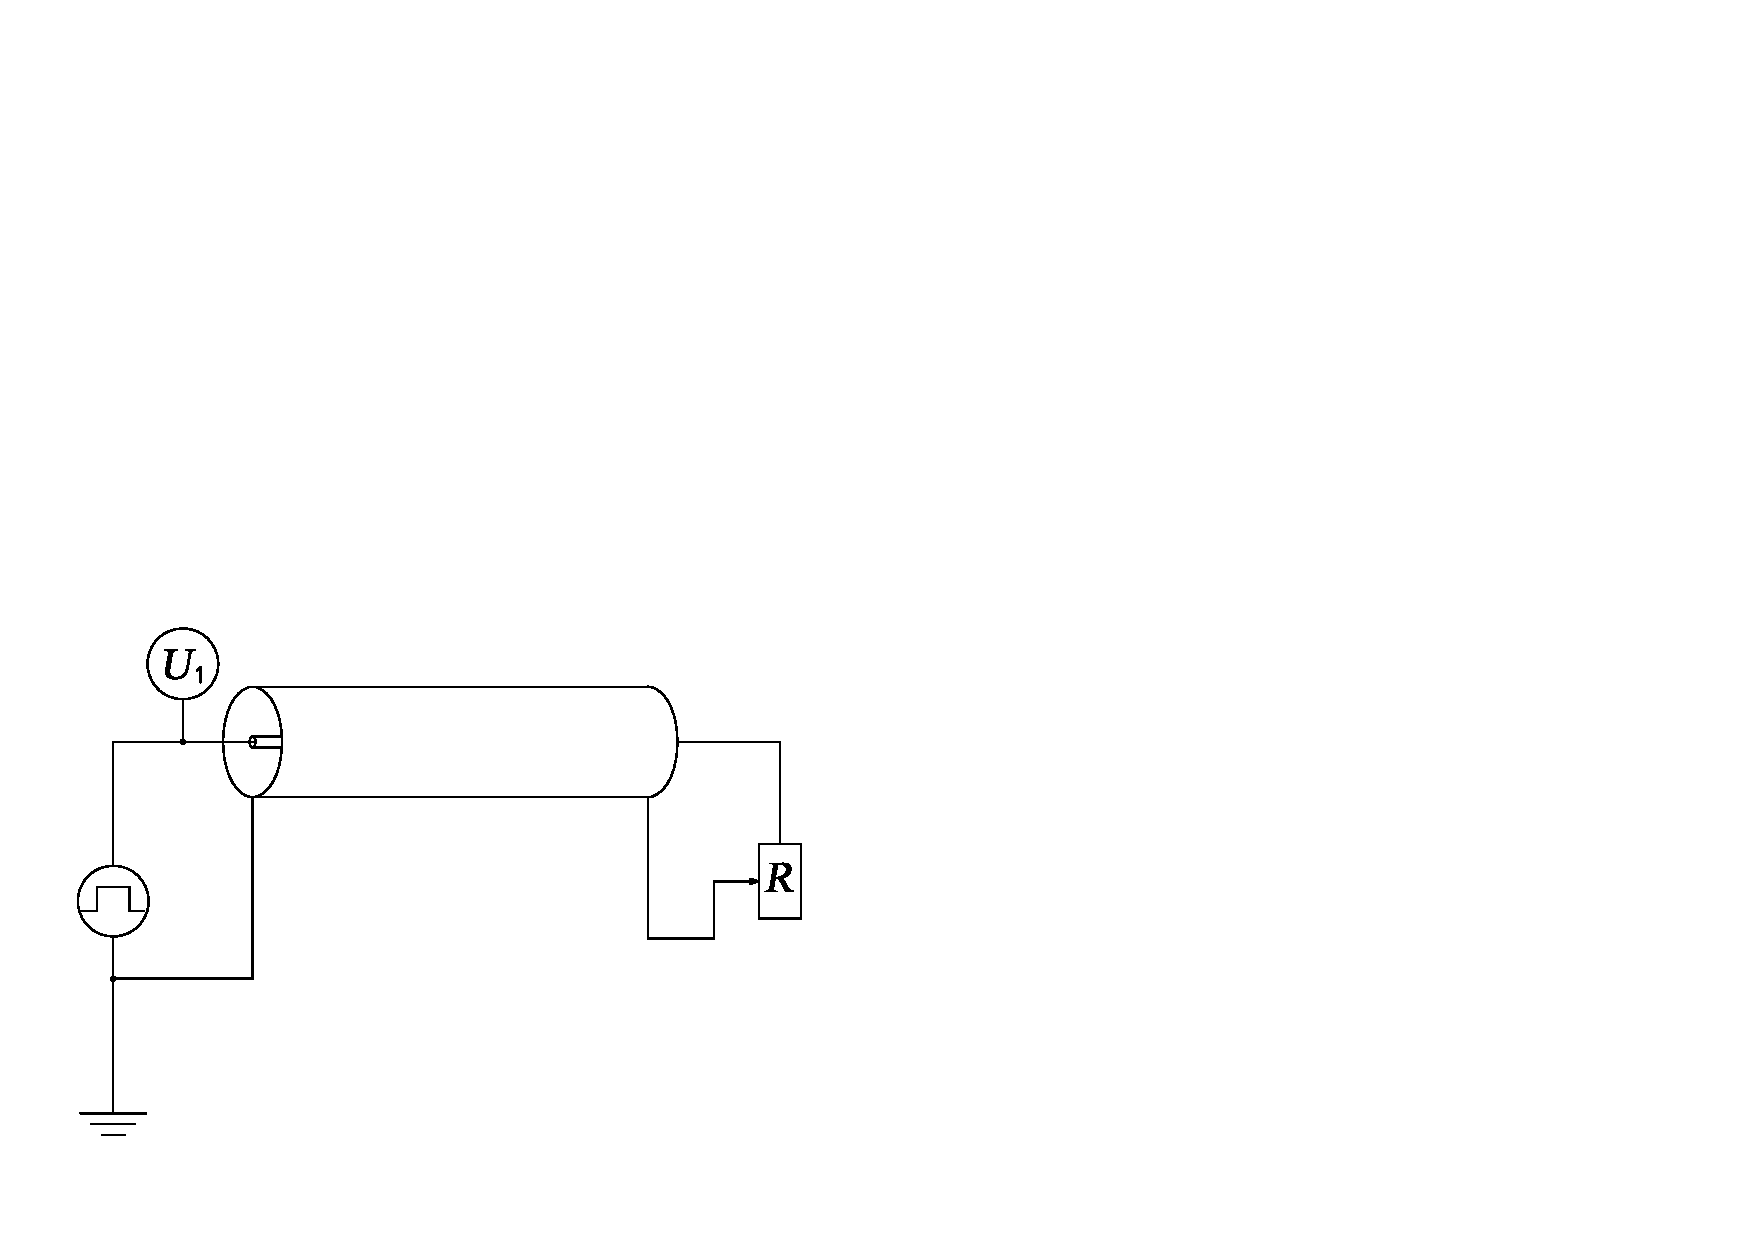
\includegraphics[width=0.7\textwidth]{Long_lines_circuit_1}
	\caption{Схема для определения волнового сопротивления кабеля}
	\label{fig:circuit_wave_r}
\end{figure}

Если не подключать ко второму концу кабеля переменное сопротивление, а оставить его разомкнутым, то на осциллографе будет видно два сигнала: сигнал, подаваемый осциллографом, и сигнал, который отразился от кабеля и вернулся. Если теперь подключить сопротивление, то, постепенно увеличивая его вплоть до некоторого значения $\omega$ можно увидеть, как сигналы постепенно сближаются, в результате чего один из них (отраженный) полностью исчезает. Это происходит в момент, когда переменное сопротивление, которое у нас выступает в роли сопротивления нагрузки, оказывается равным волновому сопротивлению кабеля.

\subsection{Определение скорости распространения волны в кабеле}

С помощью уже имеющейся у нас схемы с рисунка мы можем определить также скорость распространения волны по кабелю. Для этого второй конец кабеля вновь размыкается. После этого, с помощью изменения частоты сигнала источника, можно добиться появления на осциллографе ступенчатого сигнала (см. рисунок \ref{fig:t2theor}).

\begin{figure}[h!]
	\centering
	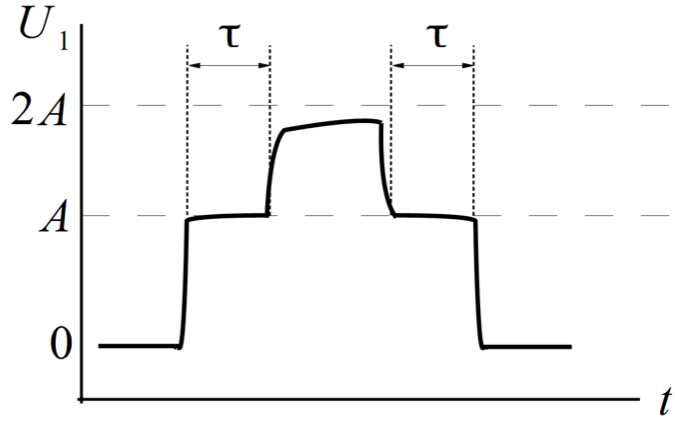
\includegraphics[width=0.5\textwidth]{Task_2_theor}        
	\caption{Сигнал на входе осциллографа при перекрытии поданного и отраженного сигналов}
	\label{fig:t2theor}
\end{figure}

Длительность ступенек (на рисунке обозначена как $\tau$) не зависит от частоты входного сигнала и определяется длиной провода и интересующей нас скоростью распространения волны следующим образом:

\begin{equation}
	\tau = 2\cdot \frac{l}{u} \qrq u =\frac{2\cdot l}{\tau}
	\label{eq:u}
\end{equation}

Здесь $l$ --- длина кабеля, $u$ --- скорость распространения волны в кабеля, $\tau$ --- ширина ступеньки по времени.

\subsection{Определение входного сопротивления кабеля в различных состояниях. Определение удельного сопротивления}

Для того, чтобы определить входное сопротивление, соберем схему, представленную на рисунке \ref{fig:circuit_rho}.

\begin{figure}[H]
	\centering
	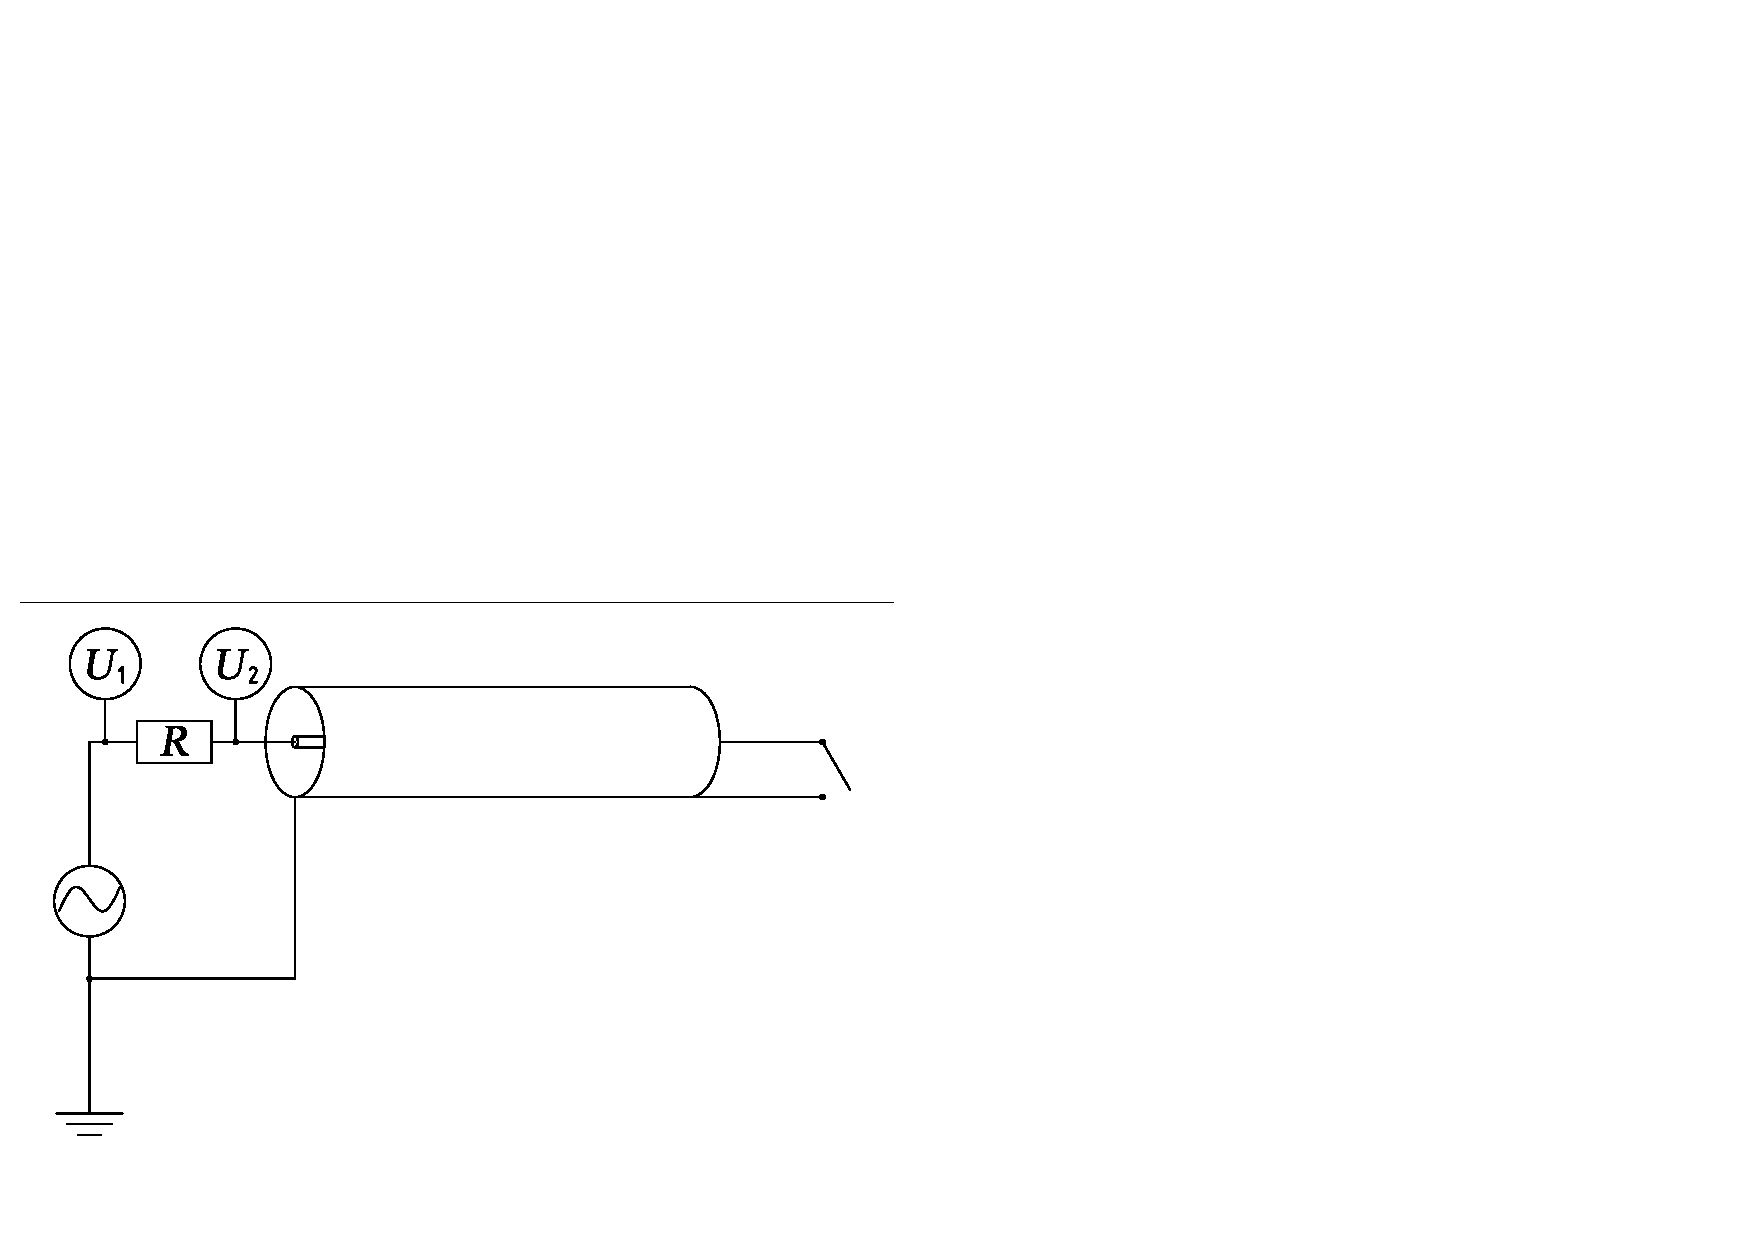
\includegraphics[width=0.7\textwidth]{Long_lines_circuit_2}
	\caption{Схема для определения погонного и удельного сопротивлений}
	\label{fig:circuit_rho}
\end{figure}

После этого, воспользовавшись предложенной программой для LabView, получим зависимость модуля входного импеданса от частоты источника. Предполагается, что получится картинка, схожая с представленной на рисунке \ref{fig:Impedance_theor}.

\begin{figure}[H]
	\centering
	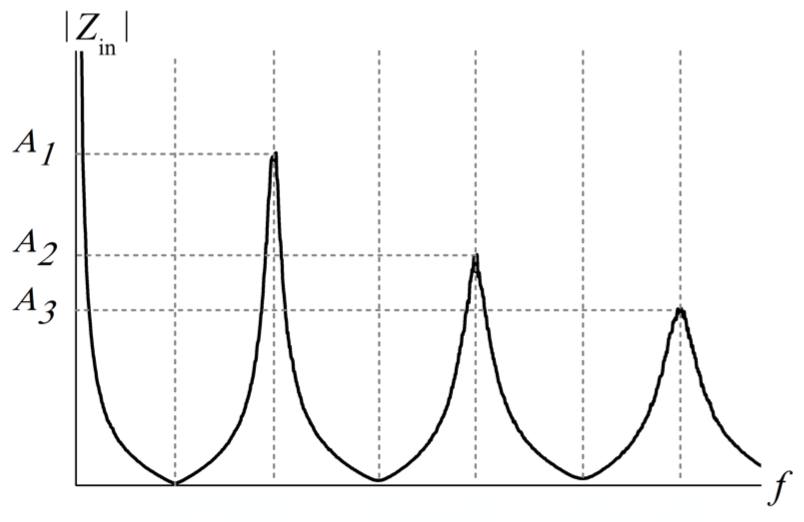
\includegraphics[width=0.6\textwidth]{Impedance_theor}
	\caption{Ожидаемая зависимость модуля импеданса от частоты источника}
	\label{fig:Impedance_theor}
\end{figure}

В видимых на рисунке максимумах значение модуля импеданса можно приблизительно выразить следующим образом:

\begin{equation*}
	|Z|_{\text{max}} \approx \frac{\Omega^2}{2 \cdot R \cdot l}
\end{equation*}

Здесь $\Omega$ --- волновое сопротивление кабеля, $l$ --- его длина, $R$ --- погонное сопротивление кабеля.

На основании этой формулы можно получить расчетную формулу для \textbf{погонного сопротивления} кабеля:

\begin{equation}
	R = \frac{\Omega^2}{2 \cdot |Z|_\text{max} \cdot l}
	\label{eq:1Resistance}
\end{equation}

Обозначения здесь такие же как и в предыдущей формуле.

Получив погонное сопротивление, для расчета \textbf{удельного сопротивления} можно воспользоваться следующей формулой:

\begin{equation*}
	R  = \frac{1}{2} \sqrt{\frac{\mu_{0}}{\pi}}\left(\frac{k_{1} \sqrt{\rho}_{1}}{a}+\frac{k_{2} \sqrt{\rho}_{2}}{b}\right) \sqrt{f}
\end{equation*}

Здесь $\mu_0$ --- магнитная постоянная, $\rho_1, \rho_2$ --- удельные сопротивления материала жилы и оплетки соответственно, $k_1, k_2$ --- параметры, определяемые геометрией изделия, $a$ --- внешний диаметр жилы, $b$ --- внутренний диаметр оплетки, $f$ --- частота источника. 

Предположим, что жила и оплетка сделаны из одного материала. Кроме того, учтем, что для кабеля с жилой, состоящей из одного провода, и сплошным экраном $k_1 = k_2 = 1$. Таким образом, получаем следующую формулу для расчета удельного сопротивления:

\begin{equation}
	\rho = \frac{4 \cdot R^2}{f} \cdot \frac{\pi}{\mu_0} \cdot \frac{a^2 \cdot b^2}{(a + b)^2}
	\label{eq:R}
\end{equation}

Здесь $\mu_0$ --- магнитная постоянная, $a$ --- внешний диаметр жилы, $b$ --- внутренний диаметр оплетки, $f$ --- частота источника, $R$ --- погонное сопротивление кабеля.

Сразу же мы можем посчитать погонную емкость провода с помощью приближенной формулы:

\begin{equation}
	C \approx \frac{56 \varepsilon}{\ln\dfrac{b}{a}}
	\label{eq:C}
\end{equation}

Отметим, что полученная емкость получается в пФ/м.

\subsection{Определение погонных сопротивления, индуктивности с помощью анализатора цепей}

Для того, чтобы определить искомые зависимости, воспользуемся анализатором цепей, каждый из концов кабеля подключается к одному из входов. В случае, когда волновое сопротивление кабеля совпадает с сопротивлением входа анализатора, мы можем определить коэффициент прохождения по формуле $S = e^{-\gamma \cdot l}$, $\gamma$ здесь --- комплексная постоянная распространения. На практике же обычно реализуется случай малых потерь, когда можно использовать упрощенное соотношение:

\begin{equation*}
	\alpha = \Re(\gamma) \approx \frac{R(f)}{2\Omega}
	\label{eq:alpha_1}
\end{equation*}

С другой стороны, посчитать коэффициент $\alpha$ можно иным способом:

\begin{equation*}
	\alpha = \Re(\gamma) = -\frac{\ln(\text{Amp}(S))}{l}
\end{equation*}

Приравняв, получаем:

\begin{equation}
	R(f) = -\frac{2\Omega}{l} \cdot \ln(\text{Amp}(S))
	\label{eq:R_pog}
\end{equation}

Теперь мы можем определить зависимость погонной индуктивности от частоты:

\begin{equation}
	L(f) = \frac{R(f)}{2\pi f} + L_b
	\label{eq:L_f}
\end{equation}

Отдельно оговорим о $L_b$, это погонная индуктивность, измеренная на больших частотах, которая в целом является постоянной величиной и может быть рассчитана по следующей формуле:

\begin{equation}
	L_b \approx 0.2 \cdot  \mu \cdot \ln \frac{b}{a}
	\label{eq:L_b}
\end{equation}

Значение $L_b$ получается в мкГн/м.

\section{Выполнение работы}

\subsection{Параметры кабеля}

Первым делом были сняты следующие параметры кабеля:

% l= 7.7 м

\begin{center}


\begin{tabular}{|c|c|c|}
	\hline 
	$a$, мм& $b$, мм  & $l$, м  \\ 
	\hline 
	0.9 & 3 & 7.7 \\ 
	\hline 
\end{tabular} 

	
\end{center}

\subsection{Определение волнового сопротивления кабеля}

В случае открытого кабеля была получена картина, представленная на рисунке \ref{fig:pt_1_open}.

\begin{figure}[H]
	\centering
	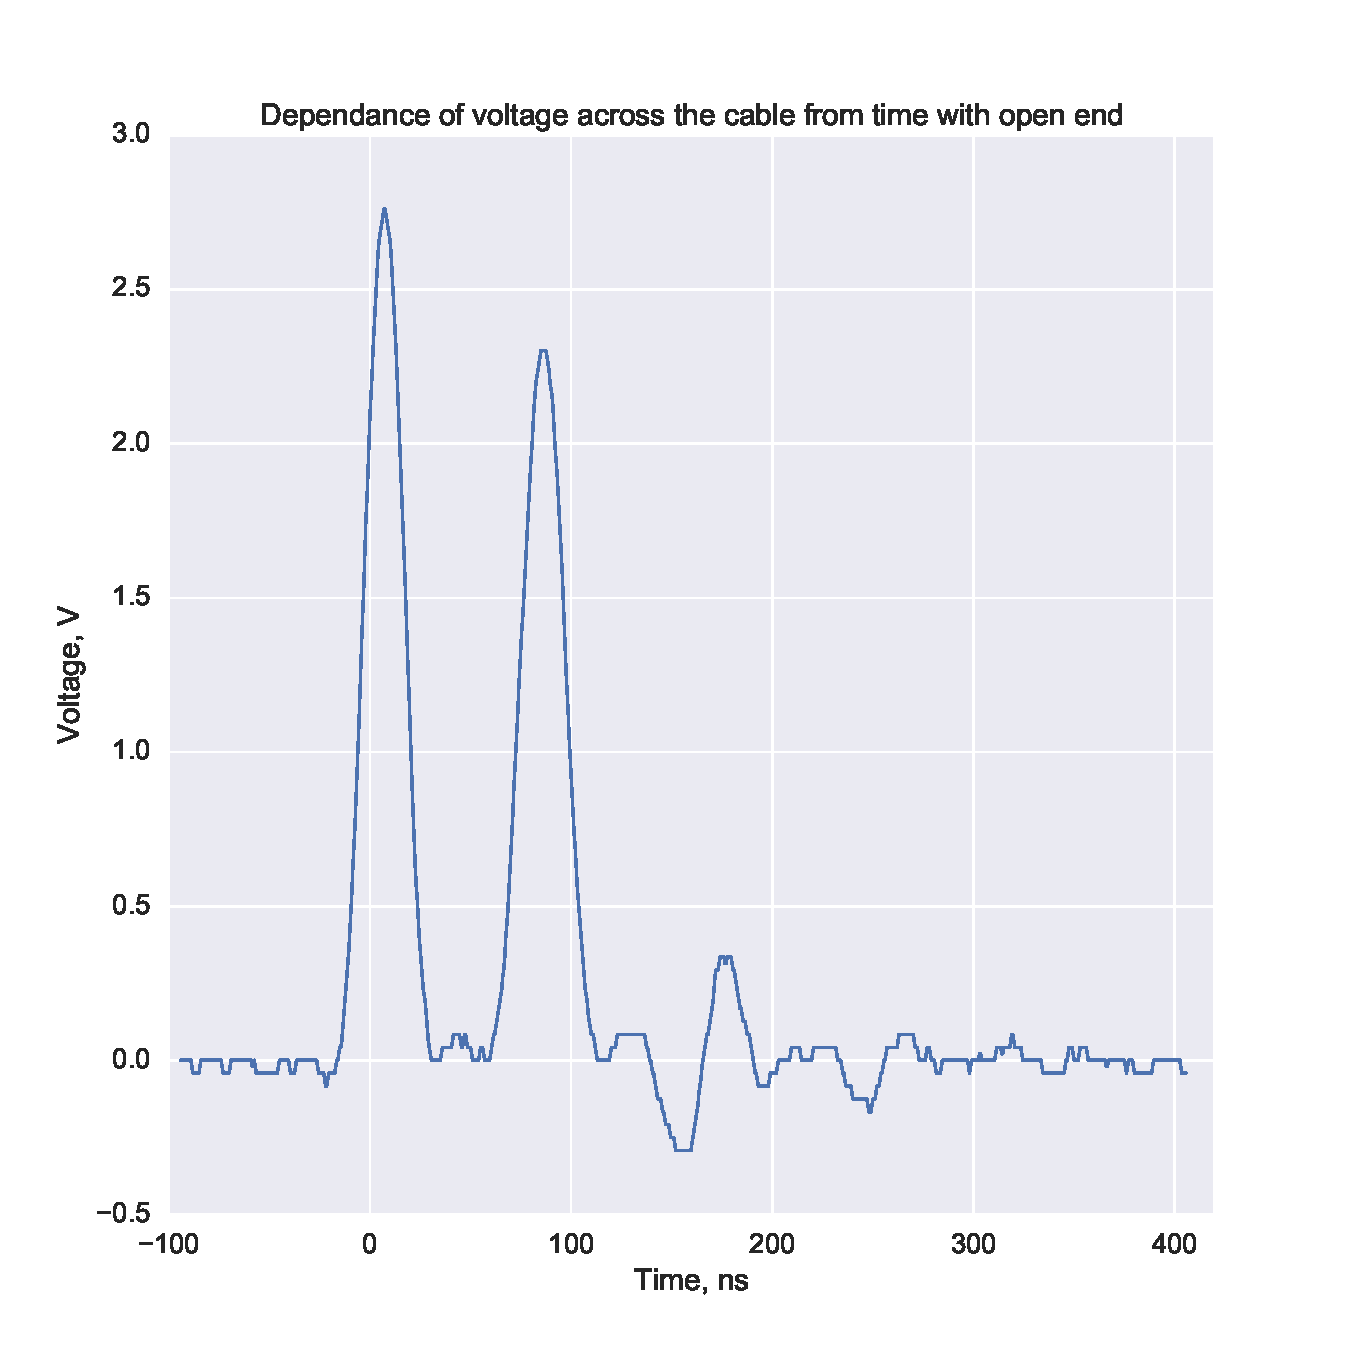
\includegraphics[width=0.7\textwidth]{pt1_open.pdf}
	\caption{Зависимость напряжения на кабеле от времени при разомкнутом конце}
	\label{fig:pt_1_open}
\end{figure}

После этого второй конец был подключен через переменное сопротивление. Меняя его вплоть до 56.1 Ома мы добились отсутствия отраженной волны, что хорошо видно на рисунке \ref{fig:pt_1_resistance}. Таким образом оказывается, что волновое сопротивление кабеля примерно равно $\boxed{\Omega = 56.1 \text{ Ом}}$

\begin{figure}[H]
	\centering
	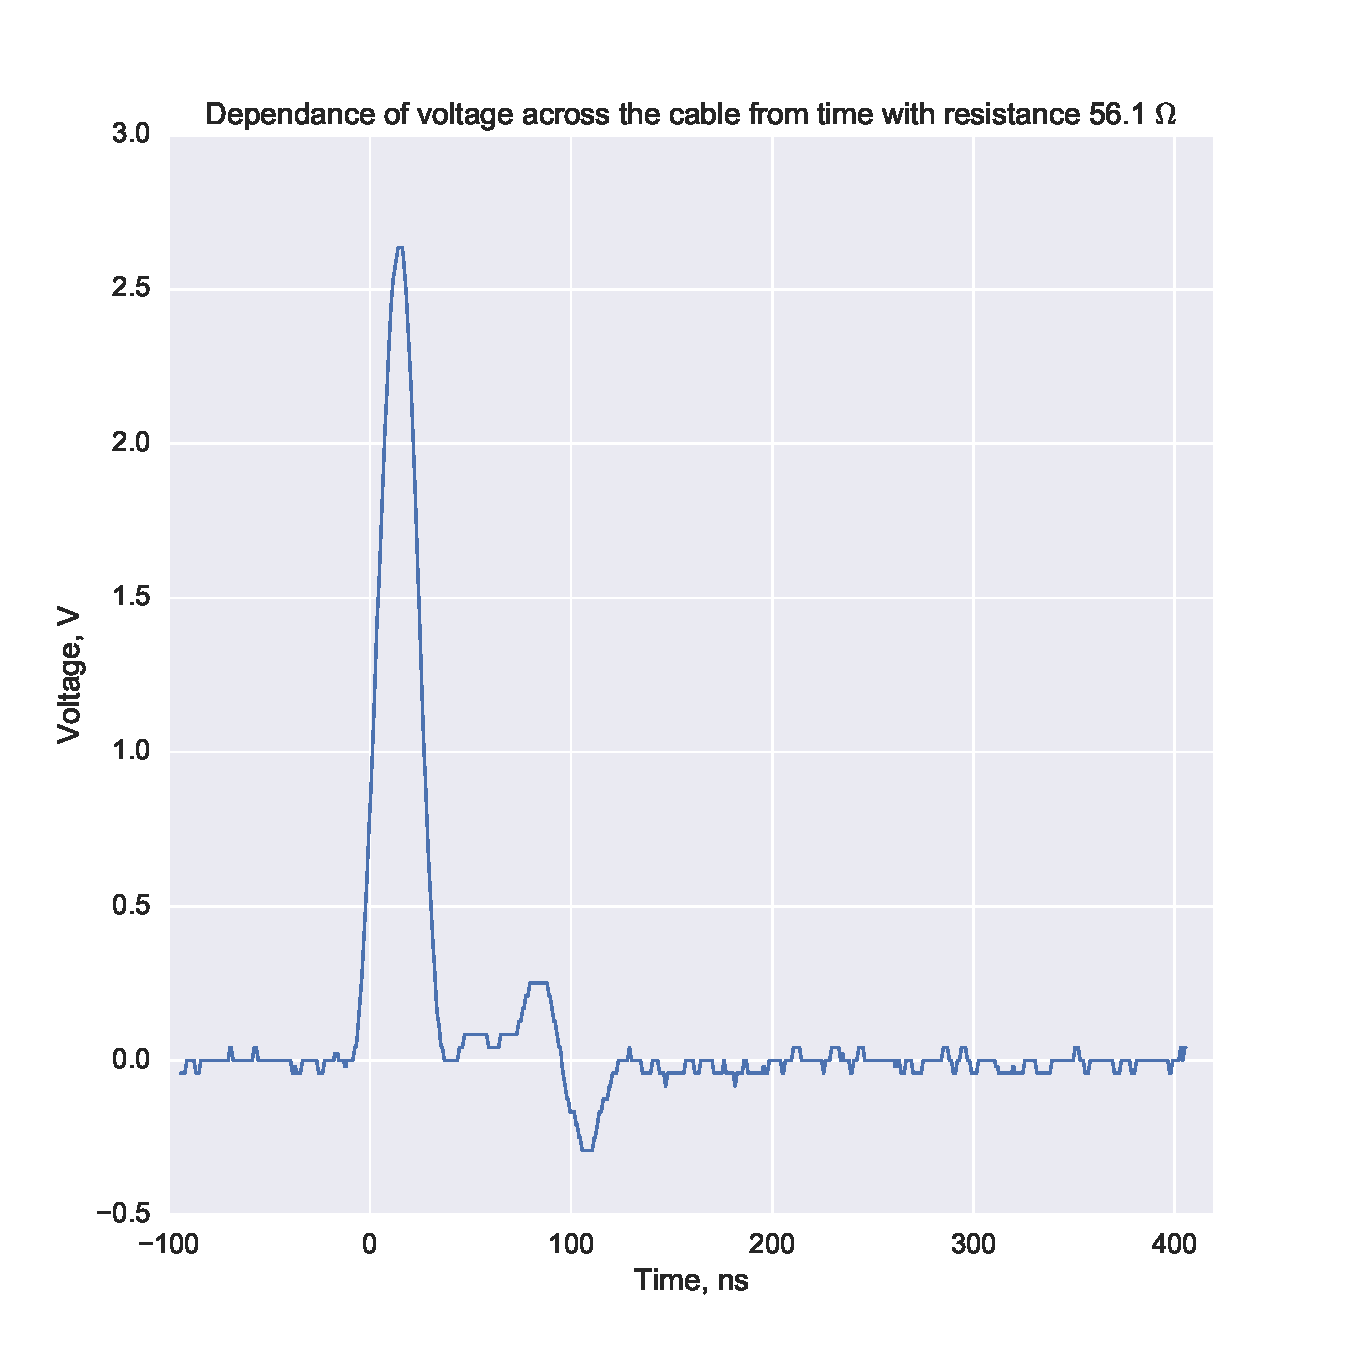
\includegraphics[width=0.7\textwidth]{pt_1_resistance.pdf}
	\caption{Зависимость напряжения на кабеле от времени при замкнутом через сопротивление 56.1 Ом конце.}
	\label{fig:pt_1_resistance}
\end{figure}

\subsection{Определение скорости распространения волны в кабеле}

После выполнения указанных действия на осциллографе была получена картина, представленная на рисунке \ref{fig:pt_2}. На основании этих данных по формуле (\ref{eq:u}) получим скорость распространения волны в кабеле $\boxed{u = 2.61 \cdot 10^8 }$ м/с. Отметим, что как и предполагалось, ширина <<ступеньки>> не зависит от частоты генератора.

\begin{figure}[H]
	\centering	
	\subfigure[]{
	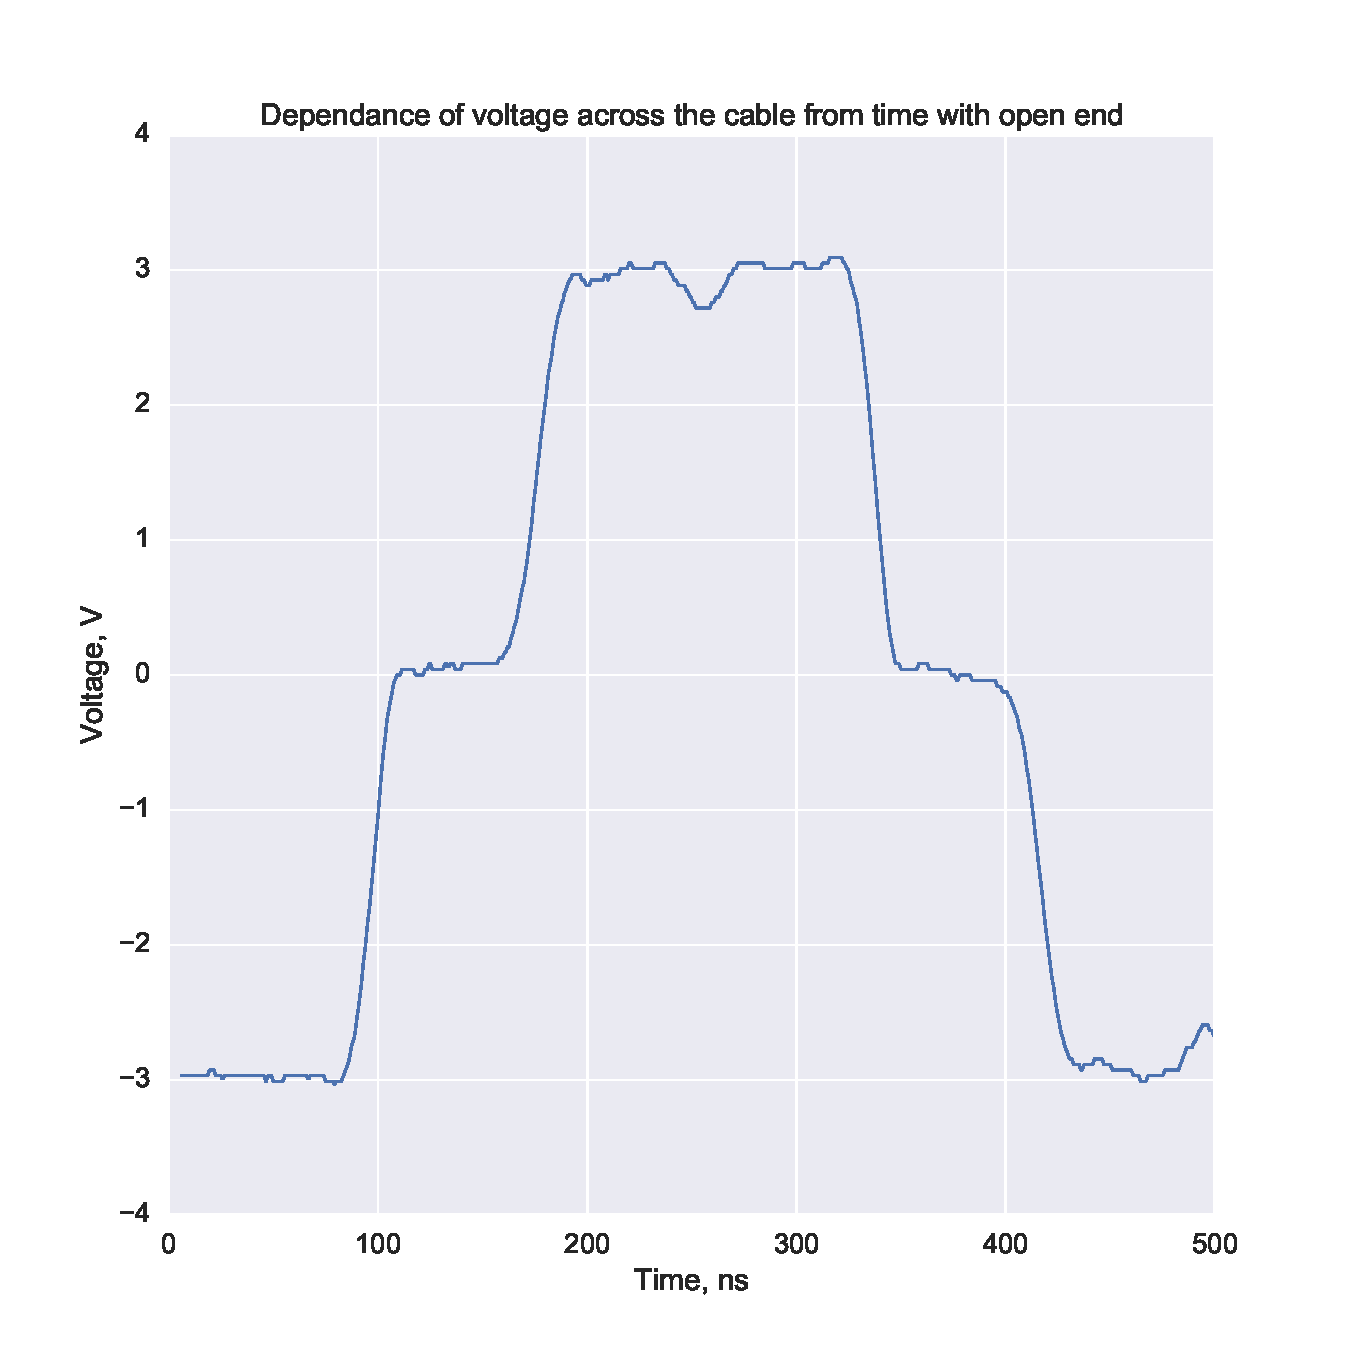
\includegraphics[width = 0.48\linewidth]{pt_2_speed.pdf}}
	\subfigure[]{
	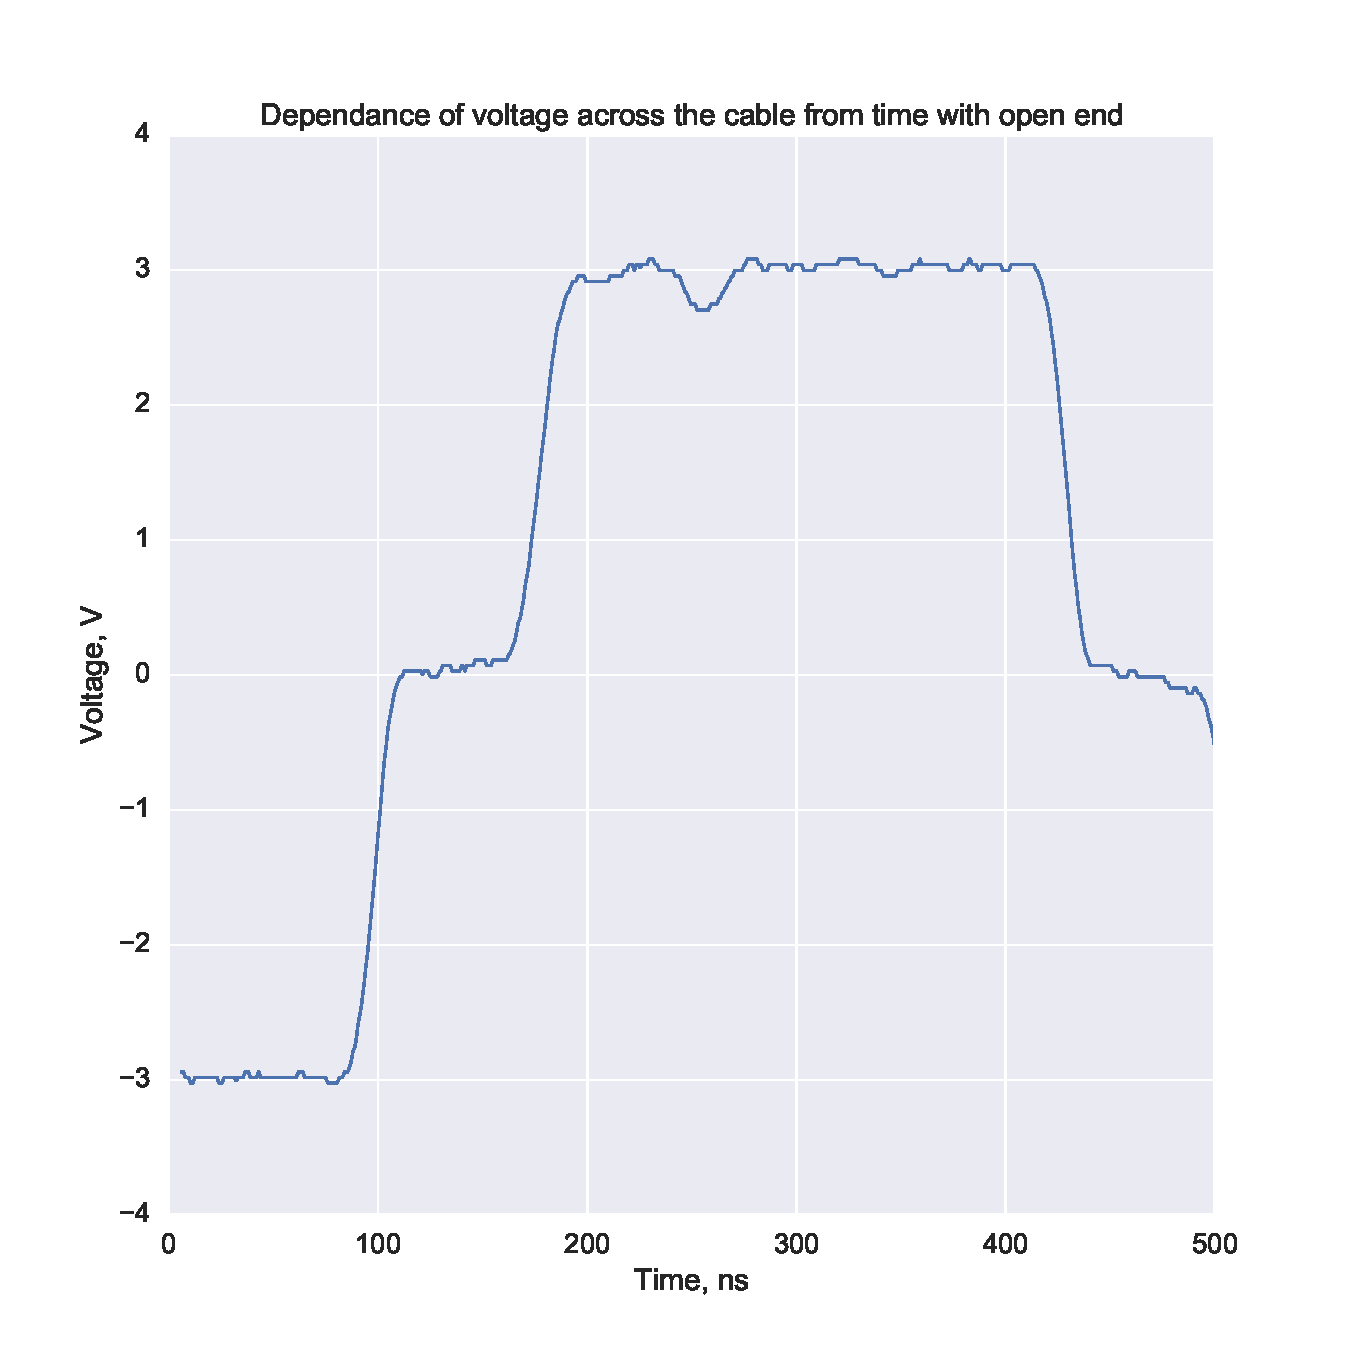
\includegraphics[width=0.48\linewidth]{pt_2_speed_1.pdf}}
	\caption{Зависимость напряжения на кабеле от времени при разомкнутом втором конце при двух различных частотах генератора.}
	\label{fig:pt_2}
\end{figure}

\subsection{Определение погонного сопротивления кабеля в различных состояниях и удельного сопротивления материала кабеля}

С помощью предоставленной программы и цепи были получены следующие наборы данных для каждого из состояний (разомкнутого, замкнутого накоротко и замкнутого на согласованную нагрузку). В нашем случае волновое сопротивление кабеля в целом оказалось равным 50 Ом, поэтому в качестве согласованной нагрузки мы использовали 50-Омный терминатор.

Полученные наборы данных представлены на рисунках \ref{fig:pt_3_1} и \ref{fig:pt_3_2}. 

\begin{figure}[H]
	\centering
	\subfigure[]{
		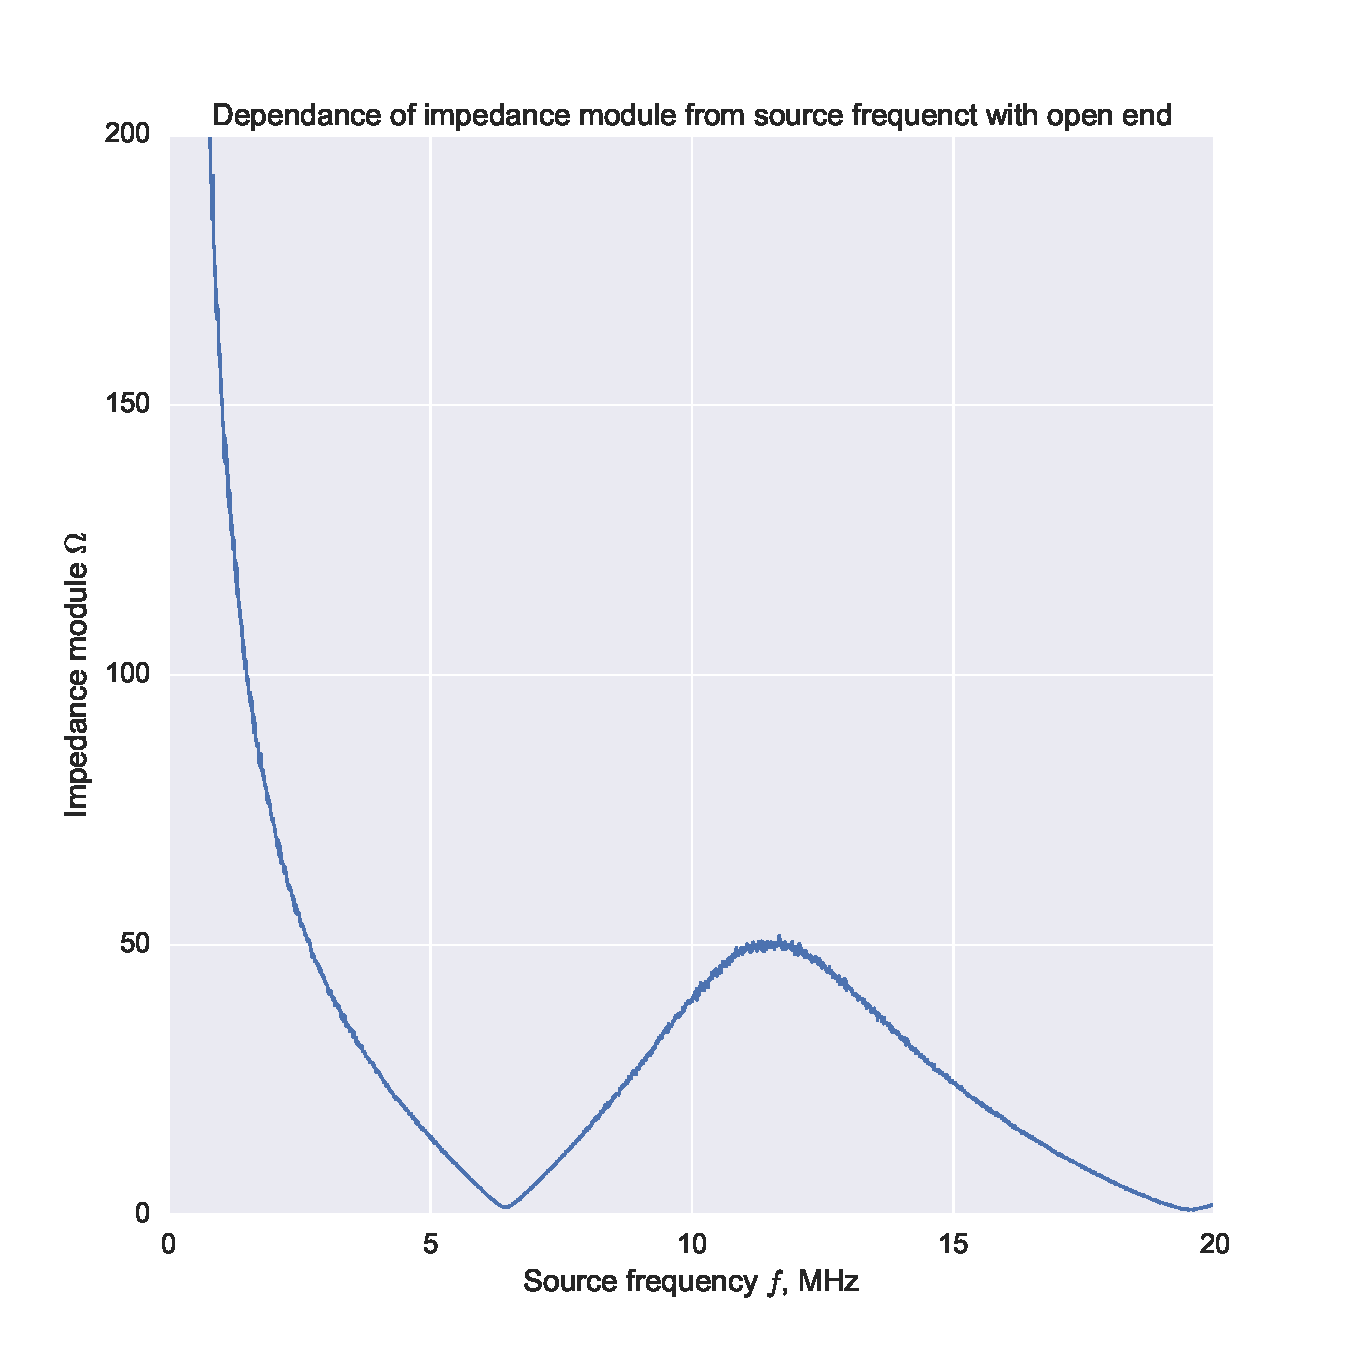
\includegraphics[width=0.48\linewidth]{pt_3_open.pdf}
		\label{fig:pt_3_open}}
	\subfigure[]{
		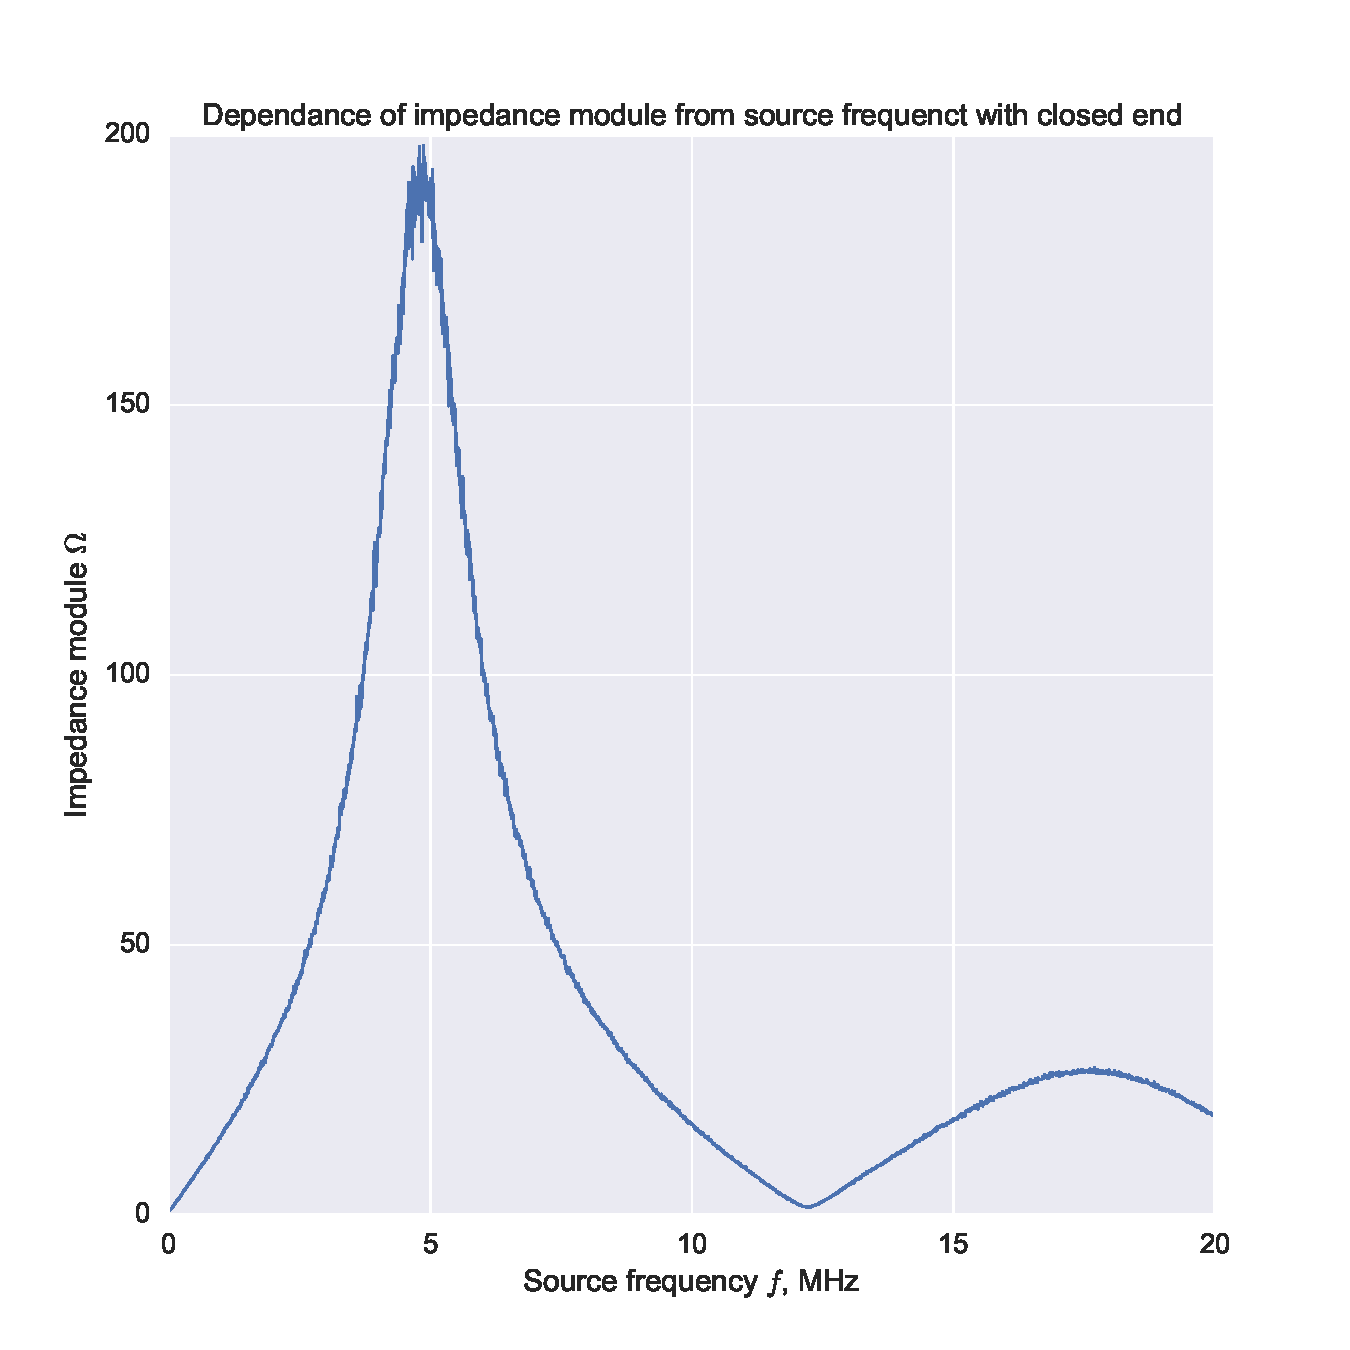
\includegraphics[width=0.48\linewidth]{pt_3_closed.pdf}
		\label{fig:pt_3_closed}}
	\caption{Зависимость модуля импеданса от частоты источника в случае разомкнутого \subref{fig:pt_3_open} и замкнутого накоротко \subref{fig:pt_3_closed} конца кабеля.}
	\label{fig:pt_3_1}
\end{figure}

\begin{figure}[H]
	\centering
	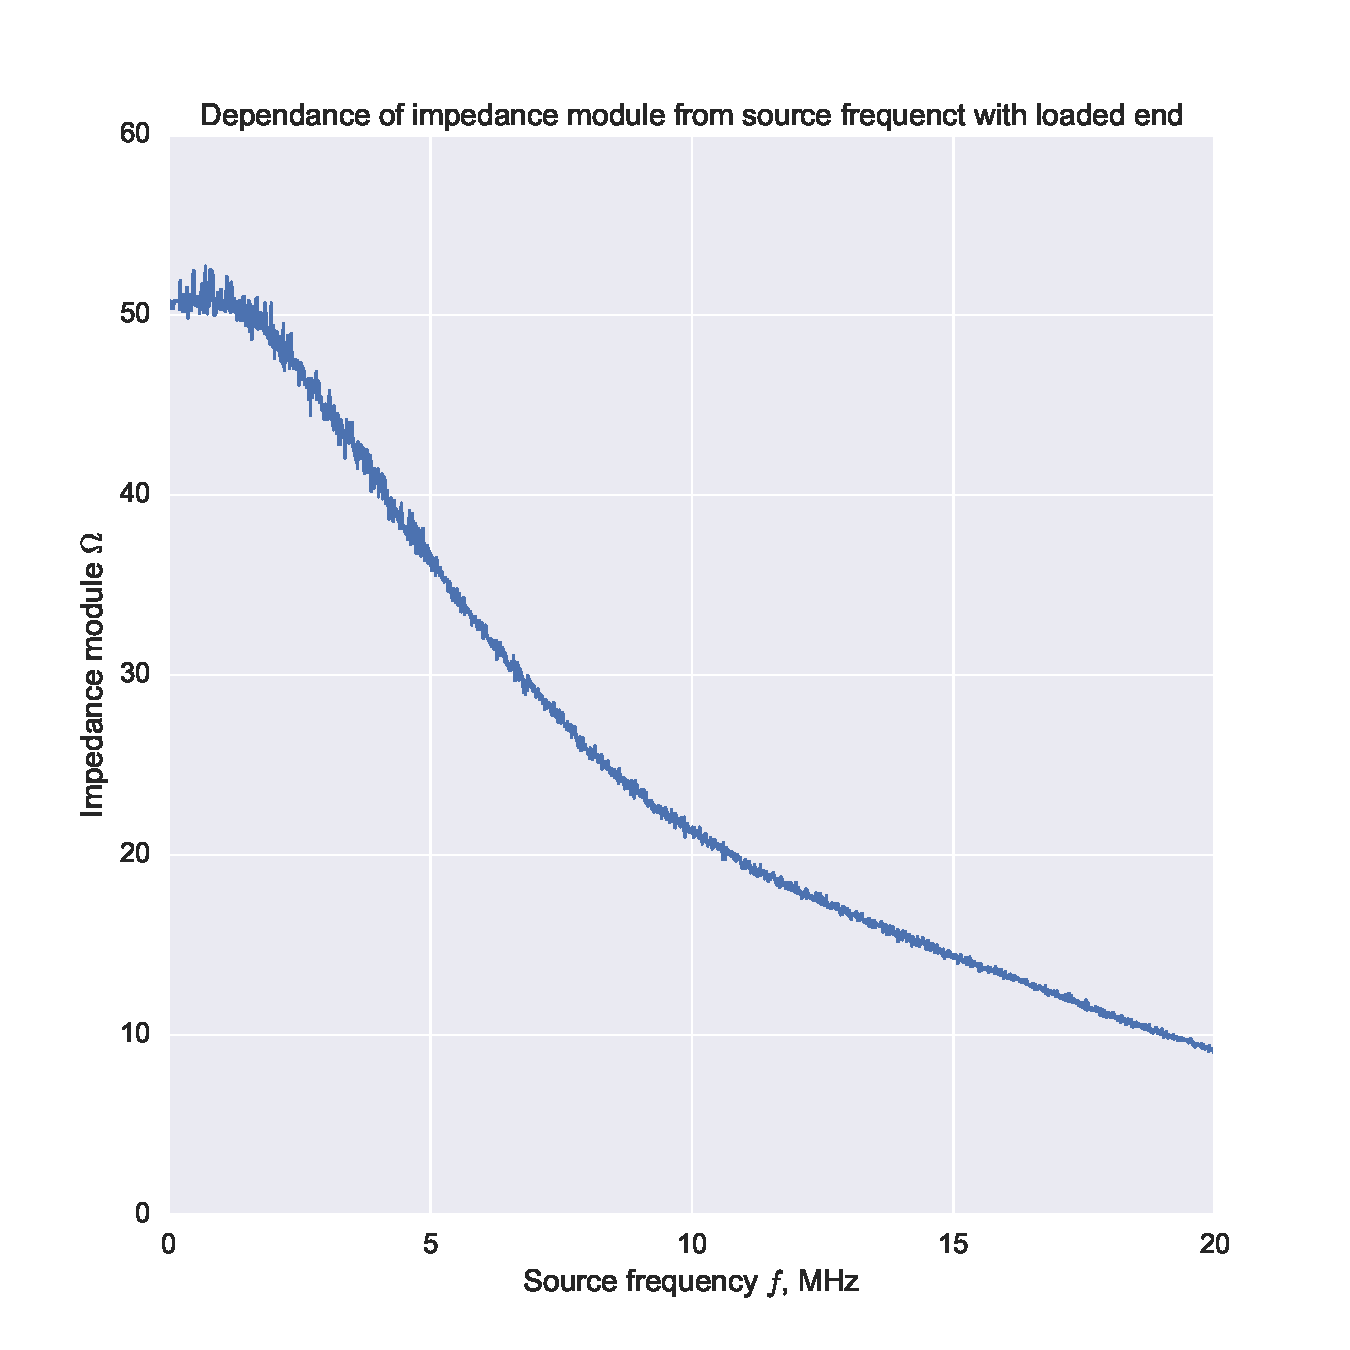
\includegraphics[width=0.48\linewidth]{pt_3_loaded.pdf}
	\caption{Зависимость модуля импеданса от частоты источника в случае замкнутого на согласованную нагрузку конца кабеля.}
	\label{fig:pt_3_2}
\end{figure}

На основании полученных данных с помощью формулы (\ref{eq:1Resistance}) и (\ref{eq:R}) было получено удельное сопротивление материала жилы, оказавшееся равным $\boxed{\rho = 4.17 \cdot 10^{-7} \text{ Ом$\cdot$м}}$.

После решения системы уравнений (\ref{eq:eqnarray_2}) получаем, что $\varepsilon = 2.3$, $\mu = 0.7$.

Здесь же также определим емкость кабеля при больших частотах с помощью формулы (\ref{eq:C}), в нашем случае равное $\boxed{C = 44.59 \text{ пФ/м}}$.

\subsection{Работа с анализатором данных}

При подключении кабеля к анализатору мы получили зависимость амплитуды коэффициента прохождения от частоты, представленную на рисунке \ref{fig:pt_4_amp}.

\begin{figure}[H]
	\centering
	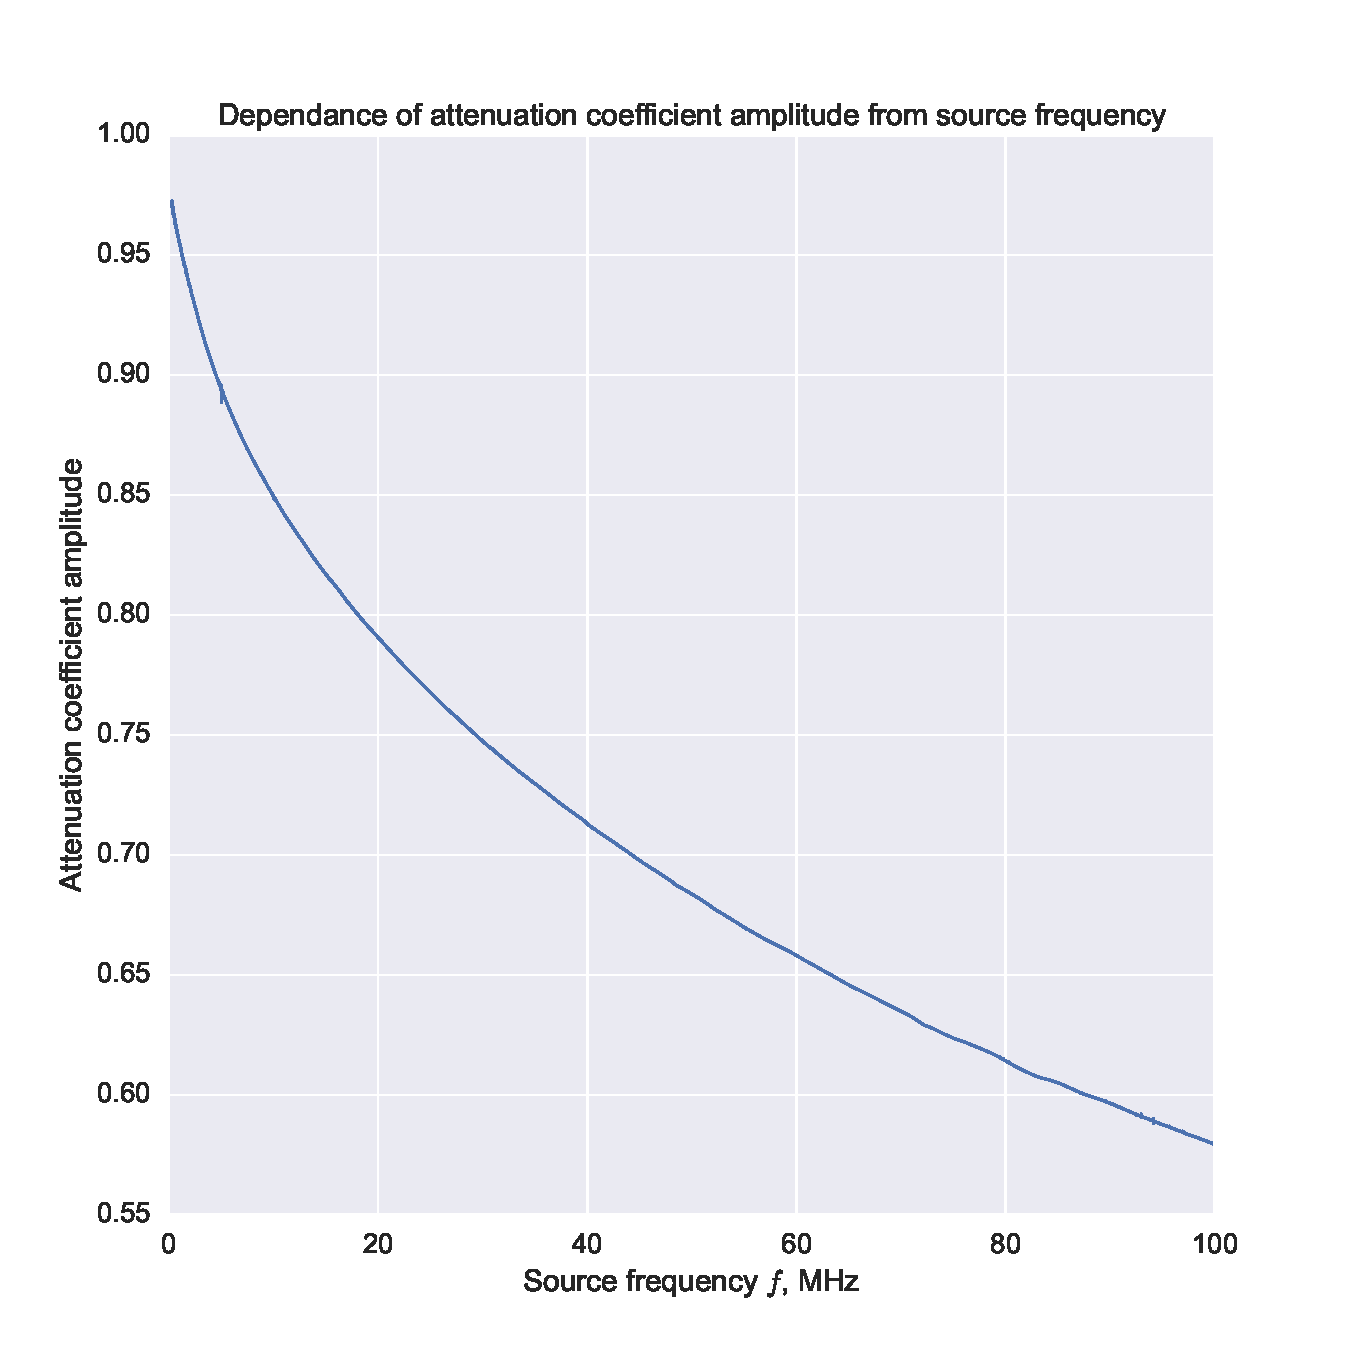
\includegraphics[width=0.7\linewidth]{pt_4.pdf}
	\caption{Зависимость амплитуды коэффициента прохождения от частоты}
	\label{fig:pt_4_amp}
\end{figure}

Воспользовавшись формулой (\ref{eq:R_pog}) мы можешь получить зависимость погонного сопротивления от частоты, которая продемонстрирована на рисунке \ref{fig:R_pog}

\begin{figure}[H]
	\centering
	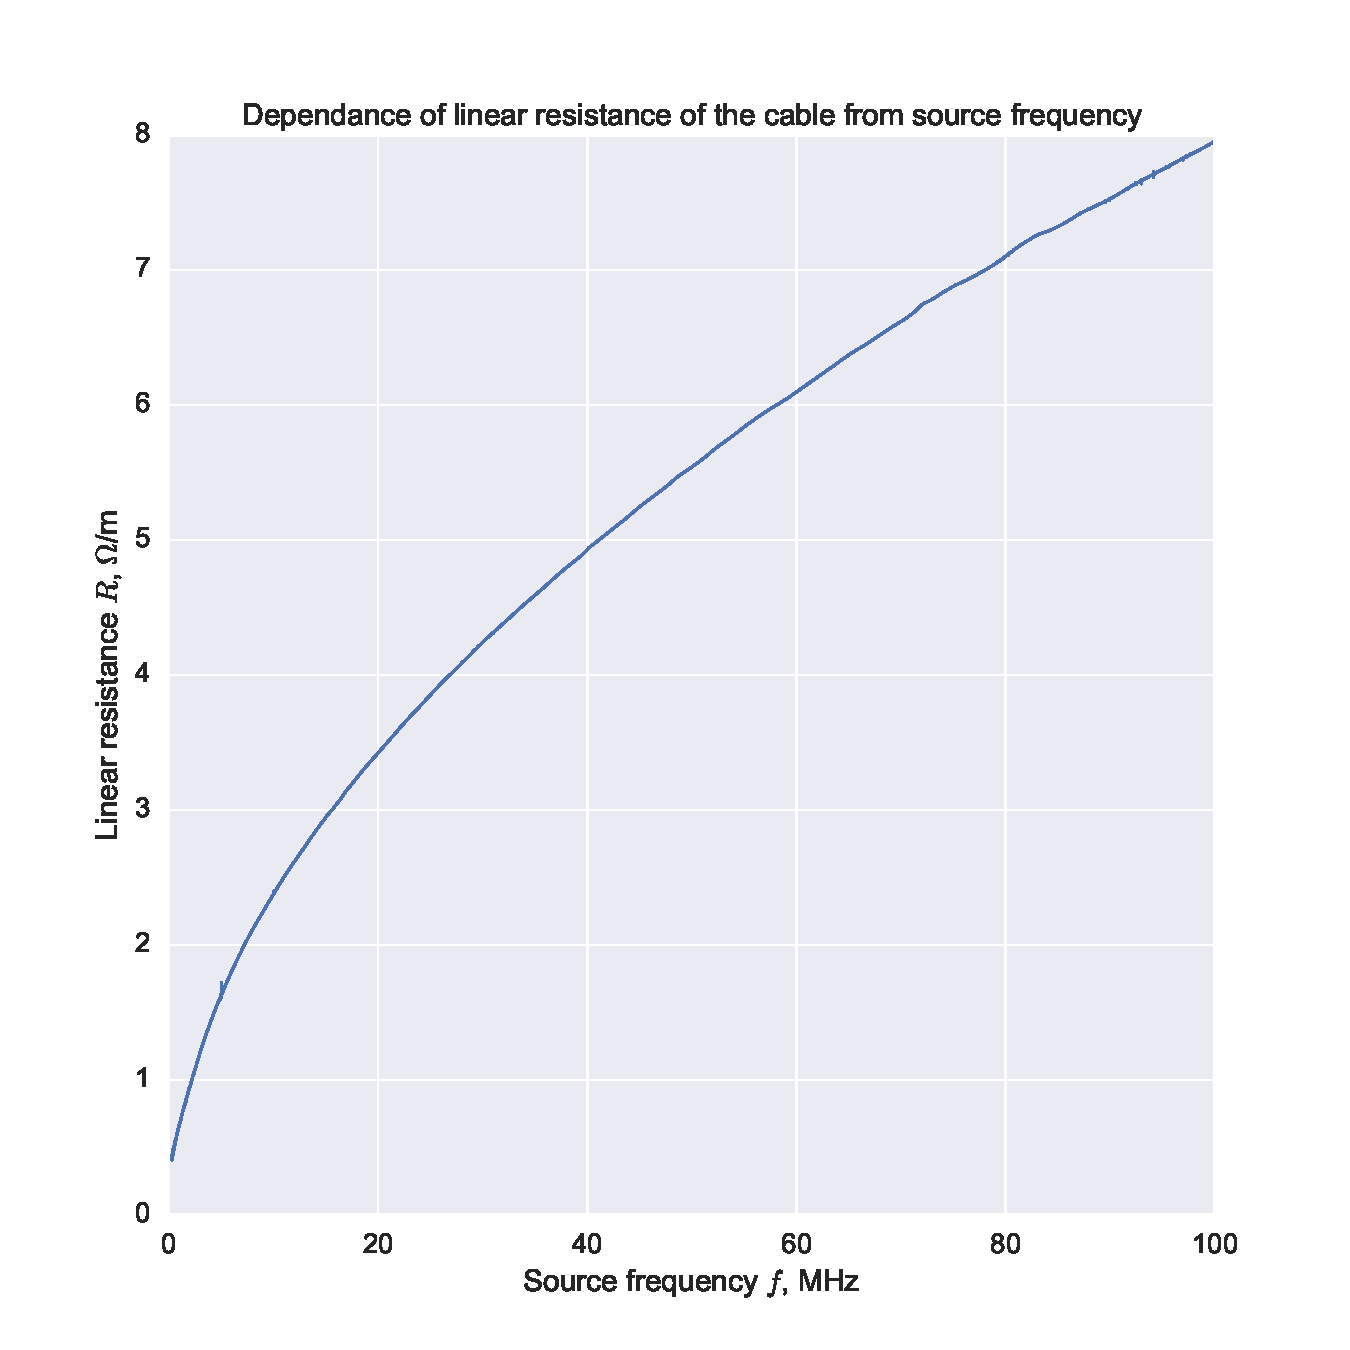
\includegraphics[width=0.7\linewidth]{pt_4_linear.pdf}
	\caption{Зависимость погонного сопротивления кабеля от частоты}
	\label{fig:R_pog}
\end{figure}

С помощью формулы (\ref{eq:L_b}) рассчитаем погонную индуктивность на больших частотах, которая оказывается равной $\boxed{L_b = 0.4 \text{ мкГн/м}}$.

Наконец, с помощью формулы (\ref{eq:L_f}) получаем зависимость погонной индуктивности от частоты. Она в свою очередь продемонстрирована на рисунке \ref{fig:L_pog}.

\begin{figure}[H]
	\centering
	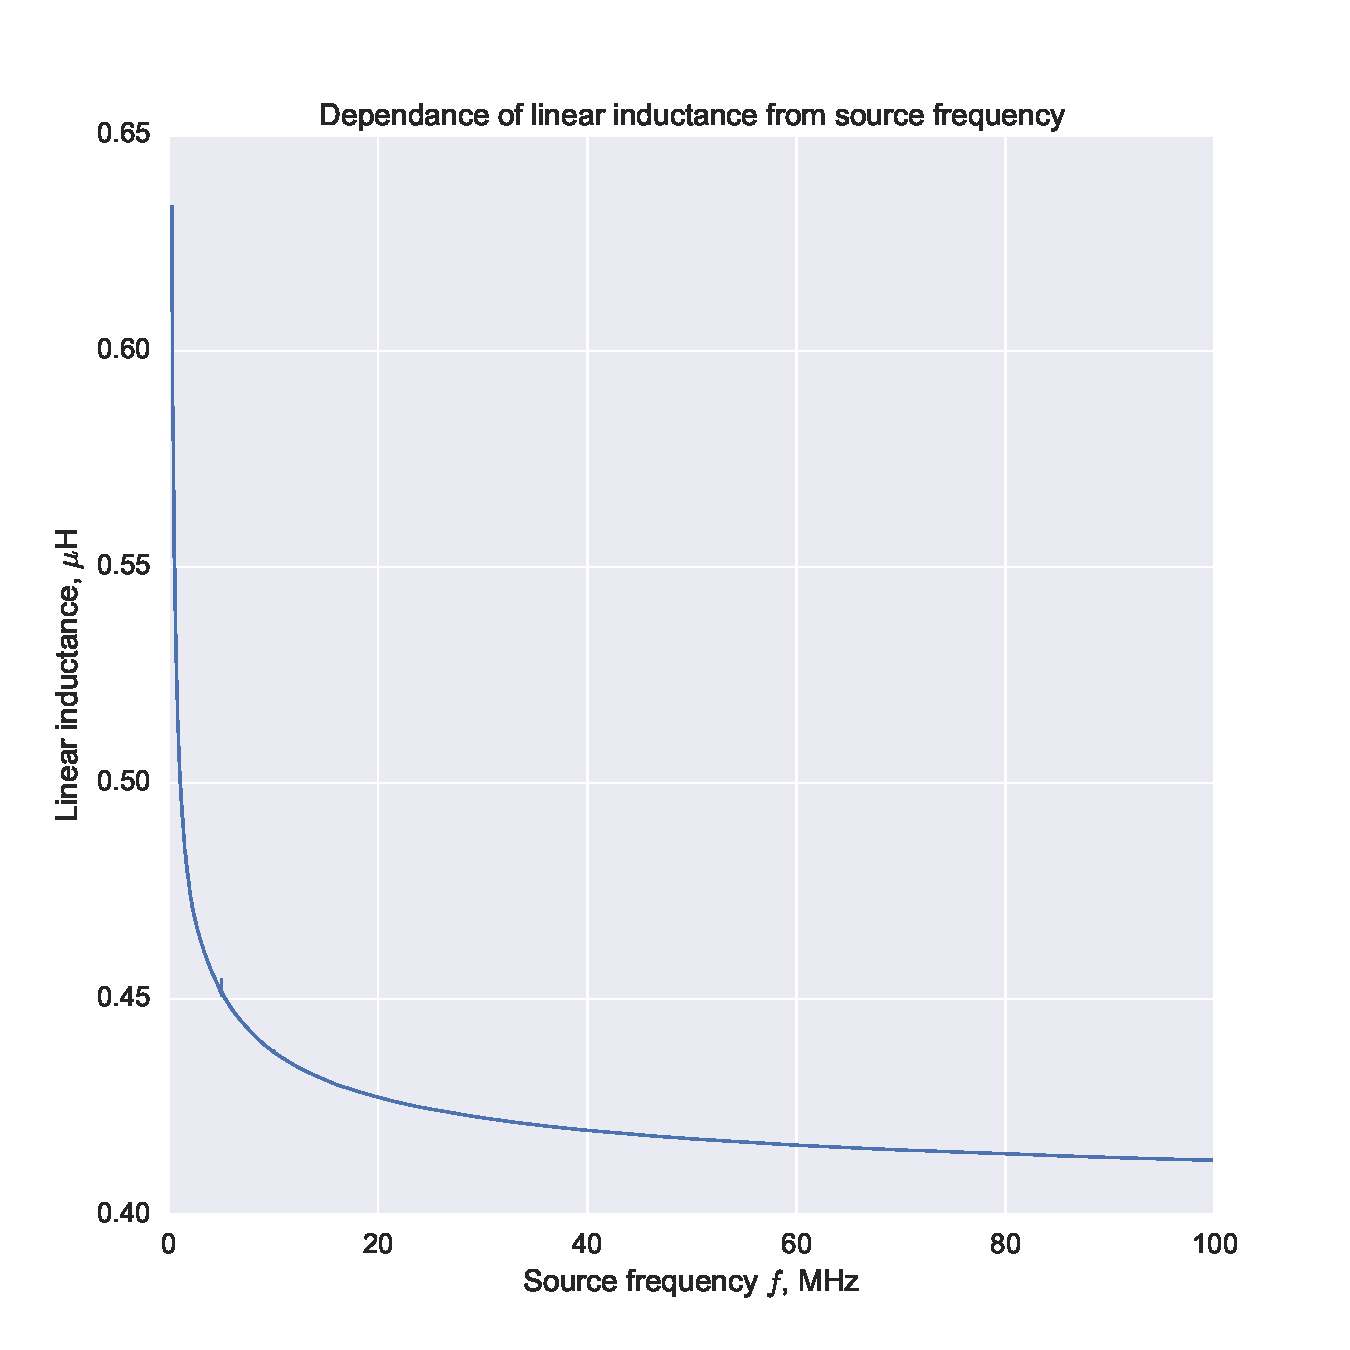
\includegraphics[width=0.7\linewidth]{pt_4_inductance.pdf}
	\caption{Зависимость погонной индуктивности кабеля от частоты}
	\label{fig:L_pog}
\end{figure}





\end{document}





















